\documentclass{beamer}
\usetheme{Madrid}
\usecolortheme{dolphin}
\setbeamertemplate{navigation symbols}{}
\setbeamercovered{transparent}
\setbeamertemplate{footline}[frame number]
\usepackage{listings}
% Packages
\usepackage{amsmath, amssymb, amsthm}
\usepackage{tikz}
\usepackage{tikz-cd}
\usetikzlibrary{arrows, positioning, matrix}


% Add this to your preamble to fix tikz-cd in Beamer
\makeatletter
\def\verbatim@nolig@list{\do\`\do\<\do\>\do\'\do\-}
\makeatother


% Title information
\title{An Introduction to Category Theory}
\subtitle{The Mathematics of Structure}
\author{Said BOUDJELDA}
\institute{Paris pantheon-assas University}
\titlegraphic{\includegraphics[width=5cm]{logo}}
\date{\today}


\begin{document}

\begin{frame}
    \titlepage
\end{frame}

\begin{frame}{Outline}
    \tableofcontents
\end{frame}

\section{Motivation and History}

\begin{frame}{Why Category Theory?}
    \begin{itemize}
        \item Originally developed in algebraic topology (1940s)
        \item Provides a unifying language for mathematics
        \item Reveals deep connections between seemingly different areas
        \item Abstracts common patterns across mathematical structures
        \item Has become increasingly important in:
            \begin{itemize}
                \item Computer science
                \item Physics
                \item Logic and foundations
            \end{itemize}
    \end{itemize}
\end{frame}

\begin{frame}{Historical Background: Before Categories}
    \begin{itemize}
        \item Mathematics was becoming increasingly abstract (1900-1940)
        \item Emmy Noether's work on abstract algebra (1920s)
            \begin{itemize}
                \item Shifted focus from specific instances to structural properties
                \item Emphasized isomorphisms over concrete representations
            \end{itemize}
        \item Topology developing rapidly
            \begin{itemize}
                \item New methods needed to classify topological spaces
                \item Algebraic invariants being developed (homology, cohomology)
            \end{itemize}
        \item Need for precise language to describe "naturality"
            \begin{itemize}
                \item Mathematicians using informal notions of "natural" mappings
                \item No formal definition of what "natural" meant
            \end{itemize}
    \end{itemize}
\end{frame}

\begin{frame}[fragile]
\frametitle{Birth of Category Theory}
    \begin{itemize}
        \item Samuel Eilenberg (topologist) and Saunders Mac Lane (algebraist)
        \item Collaboration began in 1941 at University of Michigan
        \item Working on algebraic topology problems
        \item Needed a way to formalize "natural isomorphisms"
        \item First paper: "General Theory of Natural Equivalences" (1945)
            \begin{itemize}
                \item Introduced categories, functors, and natural transformations
                \item Initially seen as a language for discussing existing concepts
            \end{itemize}
        \item Quote from Mac Lane (1996):
            \begin{quote}
                "We needed to understand natural transformations. In order to do that, we were led to formulate functors. In order to formulate functors, we needed categories."
            \end{quote}
    \end{itemize}
\end{frame}

\begin{frame}{Early Development (1945-1957)}
    \begin{itemize}
        \item Initially received with skepticism
            \begin{itemize}
                \item Derisively called "abstract nonsense" or "general abstract nonsense"
                \item Term later embraced by category theorists
            \end{itemize}
        \item Henri Cartan and Samuel Eilenberg
            \begin{itemize}
                \item Book "Homological Algebra" (1956)
                \item Used categorical language to unify and clarify concepts
            \end{itemize}
        \item Daniel Kan (1958)
            \begin{itemize}
                \item Introduced adjoint functors
                \item Significant advancement in categorical thinking
            \end{itemize}
        \item Initial applications mainly in algebraic topology and homological algebra
    \end{itemize}
\end{frame}

\begin{frame}{The Grothendieck Revolution (1957-1970)}
    \begin{itemize}
        \item Alexander Grothendieck transformed algebraic geometry
            \begin{itemize}
                \item Introduced the concept of "scheme" via categorical methods
                \item Formulated functorial approach to algebraic geometry
            \end{itemize}
        \item Tohoku paper (1957): "Sur quelques points d'algèbre homologique"
            \begin{itemize}
                \item Revolutionized homological algebra using categorical methods
                \item Introduced abelian categories
            \end{itemize}
        \item Grothendieck's seminar notes (1960s)
            \begin{itemize}
                \item Expanded category theory from a language to a foundation
                \item Developed theory of topoi and descent theory
            \end{itemize}
        \item Showed category theory could solve concrete mathematical problems
    \end{itemize}
\end{frame}

\begin{frame}{Category Theory Matures (1970s-1980s)}
    \begin{itemize}
        \item Saunders Mac Lane's "Categories for the Working Mathematician" (1971)
            \begin{itemize}
                \item First comprehensive textbook on category theory
                \item Established category theory as independent discipline
            \end{itemize}
        \item Peter Freyd and Max Kelly's contributions
            \begin{itemize}
                \item Formalization of enriched categories
                \item Development of categorical universal algebra
            \end{itemize}
        \item William Lawvere's work
            \begin{itemize}
                \item Functorial semantics for algebraic theories
                \item Elementary topos theory as foundation for mathematics
            \end{itemize}
        \item Jean Bénabou's work on bicategories and fibrations
        \item Application to logic through categorical semantics
    \end{itemize}
\end{frame}

\begin{frame}{Recent Developments (1990s-Present)}
    \begin{itemize}
        \item Expansion into computer science
            \begin{itemize}
                \item Eugenio Moggi's work on monads for programming languages
                \item Practical applications in functional programming (Haskell)
            \end{itemize}
        \item Higher category theory
            \begin{itemize}
                \item André Joyal, Ross Street, John Baez contributions
                \item Development of $n$-categories and $\infty$-categories
            \end{itemize}
        \item Homotopy Type Theory
            \begin{itemize}
                \item Vladimir Voevodsky's univalent foundations program
                \item Synthesis of type theory and homotopy theory
            \end{itemize}
        \item Applied category theory
            \begin{itemize}
                \item David Spivak, Brendan Fong, John Baez
                \item Applications to networks, databases, and complex systems
            \end{itemize}
    \end{itemize}
\end{frame}

\section{Basic Definitions}

\begin{frame}{From Sets to Categories: A Shift in Perspective}
    \begin{itemize}
        \item Traditional mathematics: Focus on objects and their internal structure
            \begin{itemize}
                \item Sets with elements
                \item Groups with operations
                \item Spaces with points
            \end{itemize}
        \item Categorical perspective: Focus on relationships between objects
            \begin{itemize}
                \item How objects relate to each other
                \item Properties defined by patterns of relationships
                \item Internal structure becomes secondary
            \end{itemize}
        \item Shift in thinking:
            \begin{itemize}
                \item From "What is it?" to "How does it behave?"
                \item From intrinsic properties to extrinsic relationships
                \item From elements to morphisms
            \end{itemize}
    \end{itemize}
\end{frame}

\begin{frame}{Philosophical Significance of Categories}
    \begin{itemize}
        \item Categories provide a "structural" view of mathematics
            \begin{itemize}
                \item Objects defined by their relationships, not internal constituents
                \item Isomorphic objects are essentially "the same"
                \item Structure preserved under transformation is what matters
            \end{itemize}
        \item Reflects structuralist philosophy in mathematics
            \begin{itemize}
                \item Mathematics studies patterns and relationships
                \item Content is secondary to structure
            \end{itemize}
        \item Beyond set theory:
            \begin{itemize}
                \item Alternative to set-theoretic foundations
                \item Captures mathematical practice more faithfully
                \item Avoids paradoxes of naive set theory
            \end{itemize}
    \end{itemize}
\end{frame}

\begin{frame}{Visualizing Categories}
    \begin{center}
        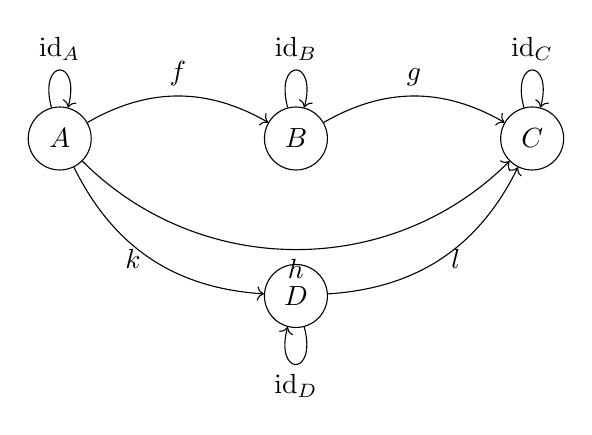
\begin{tikzpicture}
            % Objects
            \node[circle, draw, minimum size=0.8cm] (A) at (0,0) {$A$};
            \node[circle, draw, minimum size=0.8cm] (B) at (3,0) {$B$};
            \node[circle, draw, minimum size=0.8cm] (C) at (6,0) {$C$};
            \node[circle, draw, minimum size=0.8cm] (D) at (3,-2) {$D$};
            
            % Morphisms
            \draw[->] (A) to[bend left] node[above] {$f$} (B);
            \draw[->] (B) to[bend left] node[above] {$g$} (C);
            \draw[->] (A) to[bend right=45] node[below] {$h$} (C);
            \draw[->] (A) to[bend right] node[left] {$k$} (D);
            \draw[->] (D) to[bend right] node[right] {$l$} (C);
            
            % Identity morphisms
            \draw[->] (A) to[loop above] node[above] {$\text{id}_A$} (A);
            \draw[->] (B) to[loop above] node[above] {$\text{id}_B$} (B);
            \draw[->] (C) to[loop above] node[above] {$\text{id}_C$} (C);
            \draw[->] (D) to[loop below] node[below] {$\text{id}_D$} (D);
        \end{tikzpicture}
    \end{center}
    \begin{itemize}
        \item Categories can be visualized as directed graphs with identity loops
        \item Composition is represented by paths: $g \circ f$ is a path from $A$ to $C$
        \item Associativity ensures different path traversals yield the same result
        \item Identity morphisms are loops that don't change paths when composed
    \end{itemize}
\end{frame}

\begin{frame}{What is a Category?}
    \begin{definition}
        A \textbf{category} $\mathcal{C}$ consists of:
        \begin{itemize}
            \item A collection of \textbf{objects}: $\text{Ob}(\mathcal{C})$
            \item For each pair of objects $A, B$, a collection of \textbf{morphisms} (or arrows): $\text{Hom}_{\mathcal{C}}(A, B)$
            \item For each object $A$, an \textbf{identity morphism}: $\text{id}_A : A \to A$
            \item A \textbf{composition operation} for morphisms: $\circ$
        \end{itemize}
        satisfying:
        \begin{itemize}
            \item \textbf{Associativity}: $(h \circ g) \circ f = h \circ (g \circ f)$
            \item \textbf{Identity laws}: $\text{id}_B \circ f = f = f \circ \text{id}_A$ for $f: A \to B$
        \end{itemize}
    \end{definition}
\end{frame}

\begin{frame}{Examples of Categories - Part 1}
    \begin{columns}
        \begin{column}{0.5\textwidth}
            \textbf{Set} - Category of sets
            \begin{itemize}
                \item Objects: Sets
                \item Morphisms: Functions
                \item Composition: Function composition
                \item Identity: Identity function
            \end{itemize}
            
            \vspace{0.3cm}
            \textbf{Grp} - Category of groups
            \begin{itemize}
                \item Objects: Groups
                \item Morphisms: Group homomorphisms
                \item Composition: Function composition
                \item Identity: Identity homomorphism
            \end{itemize}
        \end{column}
        \begin{column}{0.5\textwidth}
            \textbf{Top} - Category of topological spaces
            \begin{itemize}
                \item Objects: Topological spaces
                \item Morphisms: Continuous maps
                \item Composition: Function composition
                \item Identity: Identity map
            \end{itemize}
            
            \vspace{0.3cm}
            \textbf{Vect$_K$} - Category of vector spaces
            \begin{itemize}
                \item Objects: Vector spaces over field $K$
                \item Morphisms: Linear transformations
                \item Composition: Function composition
                \item Identity: Identity transformation
            \end{itemize}
        \end{column}
    \end{columns}
\end{frame}

\begin{frame}{Examples of Categories - Part 2}
    \begin{columns}
        \begin{column}{0.5\textwidth}
            \textbf{Ring} - Category of rings
            \begin{itemize}
                \item Objects: Rings
                \item Morphisms: Ring homomorphisms
                \item Composition: Function composition
            \end{itemize}
            
            \vspace{0.3cm}
            \textbf{Cat} - Category of small categories
            \begin{itemize}
                \item Objects: Small categories
                \item Morphisms: Functors
                \item Composition: Functor composition
            \end{itemize}
        \end{column}
        \begin{column}{0.5\textwidth}
            \textbf{Pos} - Category of partially ordered sets
            \begin{itemize}
                \item Objects: Posets
                \item Morphisms: Order-preserving functions
                \item Composition: Function composition
            \end{itemize}
            
            \vspace{0.3cm}
            \textbf{Hask} - Category of Haskell types
            \begin{itemize}
                \item Objects: Haskell types
                \item Morphisms: Functions between types
                \item Composition: Function composition
            \end{itemize}
        \end{column}
    \end{columns}
\end{frame}

\begin{frame}{More Examples of Categories}
    \begin{itemize}
        \item \textbf{Discrete categories}:
            \begin{itemize}
                \item Only identity morphisms
                \item Example: Sets with only identity functions
            \end{itemize}
        \item \textbf{Monoids as categories}:
            \begin{itemize}
                \item A monoid can be seen as a category with just one object
                \item Morphisms correspond to monoid elements
                \item Composition corresponds to monoid operation
            \end{itemize}
        \item \textbf{Preorders as categories}:
            \begin{itemize}
                \item Objects are elements of the preorder
                \item Single morphism $a \to b$ exists iff $a \leq b$
                \item Composition follows from transitivity
            \end{itemize}
        \item \textbf{$n$ as a category}:
            \begin{itemize}
                \item Objects are numbers $0, 1, 2, \ldots, n-1$
                \item Morphism $i \to j$ exists iff $i \leq j$
            \end{itemize}
    \end{itemize}
\end{frame}

\begin{frame}{Special Types of Categories}
    \begin{itemize}
        \item \textbf{Small category}: Objects and morphisms form sets (not proper classes)
            \begin{itemize}
                \item Example: Any finite category is small
            \end{itemize}
        \item \textbf{Locally small category}: For any objects $A, B$, the morphisms $\text{Hom}(A, B)$ form a set
            \begin{itemize}
                \item Example: Most familiar categories (Set, Grp, Top)
            \end{itemize}
        \item \textbf{Discrete category}: Only identity morphisms
            \begin{itemize}
                \item Example: Sets with only identity functions
            \end{itemize}
        \item \textbf{Indiscrete/Codiscrete category}: Exactly one morphism between any two objects
            \begin{itemize}
                \item Example: Sets where all elements are related
            \end{itemize}
        \item \textbf{Thin category}: At most one morphism between any two objects
            \begin{itemize}
                \item Example: Posets as categories
            \end{itemize}
        \item \textbf{Groupoid}: Every morphism is invertible
            \begin{itemize}
                \item Example: Fundamental groupoid of a topological space
            \end{itemize}
    \end{itemize}
\end{frame}

\begin{frame}{Special Types of Morphisms - Part 1}
    \begin{columns}
        \begin{column}{0.5\textwidth}
            \textbf{Monomorphism (Mono)}
            \begin{itemize}
                \item Left-cancellative: $f \circ g_1 = f \circ g_2 \Rightarrow g_1 = g_2$
                \item Generalizes injective functions
                \item Visual: No merging of elements
                \item In Set: Precisely the injective functions
            \end{itemize}
        \end{column}
        \begin{column}{0.5\textwidth}
            \textbf{Epimorphism (Epi)}
            \begin{itemize}
                \item Right-cancellative: $g_1 \circ f = g_2 \circ f \Rightarrow g_1 = g_2$
                \item Generalizes surjective functions
                \item Visual: Covers all elements
                \item In Set: Precisely the surjective functions
            \end{itemize}
        \end{column}
    \end{columns}
    
    \vspace{0.5cm}
    Note: Monomorphism and epimorphism are dual concepts
\end{frame}

\begin{frame}{Special Types of Morphisms - Part 2}
    \begin{columns}
        \begin{column}{0.5\textwidth}
            \textbf{Isomorphism (Iso)}
            \begin{itemize}
                \item Has an inverse: $f \circ g = \text{id}$ and $g \circ f = \text{id}$
                \item Generalizes bijective functions
                \item Objects related by an isomorphism are "essentially the same" from a categorical perspective
                \item In Set: Precisely the bijective functions
            \end{itemize}
        \end{column}
        \begin{column}{0.5\textwidth}
            \textbf{Endomorphism}
            \begin{itemize}
                \item Morphism from an object to itself: $f: X \to X$
                \item Generalizes functions from a set to itself
                \item Example: Linear operators on a vector space
                \item Set of all endomorphisms forms a monoid under composition
            \end{itemize}
        \end{column}
    \end{columns}
    
    \vspace{0.3cm}
    \textbf{Automorphism}
    \begin{itemize}
        \item Isomorphism from an object to itself
        \item The set of all automorphisms of an object forms a group
        \item Example: Group of symmetries
    \end{itemize}
\end{frame}

\begin{frame}{More Special Types of Morphisms}
    \begin{itemize}
        \item \textbf{Section/Right Inverse}:
            \begin{itemize}
                \item Morphism $s: B \to A$ such that $f \circ s = \text{id}_B$
                \item In Set: Right inverse exists iff $f$ is surjective
            \end{itemize}
        \item \textbf{Retraction/Left Inverse}:
            \begin{itemize}
                \item Morphism $r: B \to A$ such that $r \circ f = \text{id}_A$
                \item In Set: Left inverse exists iff $f$ is injective
            \end{itemize}
        \item \textbf{Bimorphism}:
            \begin{itemize}
                \item Both a monomorphism and an epimorphism
                \item Not necessarily an isomorphism (unlike in Set)
            \end{itemize}
        \item \textbf{Zero morphism}:
            \begin{itemize}
                \item In categories with zero objects, a morphism that factors through the zero object
                \item Example: Zero matrix in Vect$_K$
            \end{itemize}
    \end{itemize}
\end{frame}

\begin{frame}[fragile]
    \frametitle{Natural Transformations}
    \begin{definition}
        A \textbf{natural transformation} $\eta: F \Rightarrow G$ between functors $F, G: \mathcal{C} \to \mathcal{D}$ consists of:
        \begin{itemize}
            \item For each object $X$ in $\mathcal{C}$, a morphism $\eta_X: F(X) \to G(X)$ in $\mathcal{D}$
        \end{itemize}
        such that for every morphism $f: X \to Y$ in $\mathcal{C}$, the following diagram commutes:
        \begin{center}
            \begin{tikzcd}
                F(X) \arrow[r, "F(f)"] \arrow[d, "\eta_X"'] & F(Y) \arrow[d, "\eta_Y"] \\
                G(X) \arrow[r, "G(f)"']                      & G(Y)
            \end{tikzcd}
        \end{center}
        (i.e., $\eta_Y \circ F(f) = G(f) \circ \eta_X$)
    \end{definition}
\end{frame}

\begin{frame}[fragile]
\frametitle{Natural Isomorphisms}
    \begin{definition}
        A \textbf{natural isomorphism} is a natural transformation $\eta: F \Rightarrow G$ where each component $\eta_X$ is an isomorphism.
    \end{definition}
    
    \begin{center}
        \begin{tikzcd}
            F(X) \arrow[r, "F(f)"] \arrow[d, "\eta_X"', "\cong"] & F(Y) \arrow[d, "\eta_Y", "\cong"'] \\
            G(X) \arrow[r, "G(f)"']                               & G(Y)
        \end{tikzcd}
    \end{center}
    
    \begin{itemize}
        \item Represents a structure-preserving equivalence between functors
        \item Captures when two functorial constructions are "essentially the same"
        \item Example: For finite-dimensional vector spaces $V$, the natural isomorphism $V \cong (V^*)^*$
    \end{itemize}
\end{frame}

\section{Universal Properties and Limits}

\begin{frame}{Universal Properties}
    \begin{itemize}
        \item Define objects by how they relate to other objects
        \item Characterize objects up to unique isomorphism
        \item Examples:
            \begin{itemize}
                \item Products and coproducts
                \item Equalizers and coequalizers
                \item Pullbacks and pushouts
                \item Initial and terminal objects
            \end{itemize}
        \item Unify constructions across different categories
    \end{itemize}
\end{frame}

\begin{frame}[fragile]
    \frametitle{Products and Coproducts}
    \begin{columns}
        \begin{column}{0.5\textwidth}
            \textbf{Product} of $A$ and $B$:
            \begin{center}
                \begin{tikzcd}
                    & P \arrow[dl, "p_1"'] \arrow[dr, "p_2"] & \\
                    A & & B
                \end{tikzcd}
            \end{center}
            
            With universal property:
            \begin{center}
                \begin{tikzcd}
                    & X \arrow[d, dashed, "\exists! u"] \arrow[dl, "f"'] \arrow[dr, "g"] & \\
                    A & P \arrow[l, "p_1"] \arrow[r, "p_2"'] & B
                \end{tikzcd}
            \end{center}
        \end{column}
        \begin{column}{0.5\textwidth}
            \textbf{Coproduct} of $A$ and $B$:
            \begin{center}
                \begin{tikzcd}
                    & C & \\
                    A \arrow[ur, "i_1"] & & B \arrow[ul, "i_2"']
                \end{tikzcd}
            \end{center}
            
            With universal property:
            \begin{center}
                \begin{tikzcd}
                    & C \arrow[d, dashed, "\exists! u"] & \\
                    A \arrow[ur, "i_1"] \arrow[dr, "f"'] & & B \arrow[ul, "i_2"'] \arrow[dl, "g"] \\
                    & X &
                \end{tikzcd}
            \end{center}
        \end{column}
    \end{columns}
\end{frame}

\begin{frame}{Examples of Products and Coproducts}
    \begin{columns}
        \begin{column}{0.5\textwidth}
            \textbf{Products}
            \begin{itemize}
                \item \textbf{Set}: Cartesian product with projections
                \item \textbf{Grp}: Direct product with projections
                \item \textbf{Top}: Product space with projections
                \item \textbf{Vect$_K$}: Direct sum with projections
            \end{itemize}
        \end{column}
        \begin{column}{0.5\textwidth}
            \textbf{Coproducts}
            \begin{itemize}
                \item \textbf{Set}: Disjoint union with inclusions
                \item \textbf{Grp}: Free product with inclusions
                \item \textbf{Top}: Disjoint union with inclusions
                \item \textbf{Vect$_K$}: Direct sum with inclusions
            \end{itemize}
        \end{column}
    \end{columns}
\end{frame}

\begin{frame}{Limits and Colimits}
    \begin{itemize}
        \item \textbf{Diagram}: A functor $D: \mathcal{J} \to \mathcal{C}$ from a small index category
        \item \textbf{Cone}: An object $X$ with morphisms to each object in the diagram, commuting with diagram arrows
        \item \textbf{Limit}: The universal cone
        \item \textbf{Colimit}: The universal cocone (dual notion)
    \end{itemize}
    
    Examples of limits:
    \begin{itemize}
        \item Terminal object: Limit of empty diagram
        \item Product: Limit of discrete diagram
        \item Equalizer: Limit of parallel arrows
        \item Pullback: Limit of span diagram
    \end{itemize}
\end{frame}

\section{Adjunctions and Monads}

\begin{frame}{Adjunctions}
    \begin{definition}
        An \textbf{adjunction} between categories $\mathcal{C}$ and $\mathcal{D}$ consists of functors $F: \mathcal{C} \to \mathcal{D}$ and $G: \mathcal{D} \to \mathcal{C}$, together with a natural bijection:
        \[\text{Hom}_{\mathcal{D}}(F(A), B) \cong \text{Hom}_{\mathcal{C}}(A, G(B))\]
        for all objects $A$ in $\mathcal{C}$ and $B$ in $\mathcal{D}$.
        
        We write $F \dashv G$ and say "$F$ is left adjoint to $G$" or "$G$ is right adjoint to $F$".
    \end{definition}
\end{frame}

\begin{frame}[fragile]
\frametitle{Adjunctions: Unit and Counit}
    Equivalently, an adjunction can be defined by two natural transformations:
    \begin{itemize}
        \item \textbf{Unit}: $\eta: 1_{\mathcal{C}} \Rightarrow G \circ F$
        \item \textbf{Counit}: $\varepsilon: F \circ G \Rightarrow 1_{\mathcal{D}}$
    \end{itemize}
    
    Satisfying the triangle identities:
    \begin{columns}
        \begin{column}{0.5\textwidth}
            \begin{tikzcd}
                F \arrow[r, "F\eta"] \arrow[dr, equal] & FGF \arrow[d, "\varepsilon F"] \\
                & F
            \end{tikzcd}
        \end{column}
        \begin{column}{0.5\textwidth}
            \begin{tikzcd}
                G \arrow[r, "\eta G"] \arrow[dr, equal] & GFG \arrow[d, "G\varepsilon"] \\
                & G
            \end{tikzcd}
        \end{column}
    \end{columns}
\end{frame}

\begin{frame}{Examples of Adjunctions}
    \begin{itemize}
        \item \textbf{Free-Forgetful adjunction}:
            \begin{itemize}
                \item Free functor $F: \textbf{Set} \to \textbf{Grp}$ 
                \item Forgetful functor $U: \textbf{Grp} \to \textbf{Set}$
                \item $F \dashv U$
            \end{itemize}
        \item \textbf{Product-Diagonal adjunction}:
            \begin{itemize}
                % \item Product functor $- \times A: \textbf{Set} \to \textbf
                \item Diagonal functor $\Delta: \textbf{Set} \to \textbf{Set} \times \textbf{Set}$
                \item $- \times A \dashv \Delta$
            \end{itemize}
        \item \textbf{Currying adjunction}:
            \begin{itemize}
                \item $-\times B \dashv (-)^B$ in cartesian closed categories
                \item Captures currying in lambda calculus
            \end{itemize}
        \item \textbf{Stone-Čech compactification}:
            \begin{itemize}
                \item Left adjoint to the forgetful functor from compact Hausdorff spaces to topological spaces
            \end{itemize}
        \item \textbf{Galois connections}:
            \begin{itemize}
                \item Special case of adjunctions between poset categories
            \end{itemize}
    \end{itemize}
    \end{frame}
    
    \begin{frame}[fragile]
    \frametitle{Monads}
    \begin{definition}
    A \textbf{monad} on a category $\mathcal{C}$ consists of:
    \begin{itemize}
        \item An endofunctor $T: \mathcal{C} \to \mathcal{C}$
        \item A unit natural transformation $\eta: 1_{\mathcal{C}} \Rightarrow T$
        \item A multiplication natural transformation $\mu: T^2 \Rightarrow T$
    \end{itemize}
    satisfying the following coherence conditions:
    \begin{columns}
        \begin{column}{0.5\textwidth}
            \begin{center}
                (Associativity)
                \begin{tikzcd}
                    T^3 \arrow[r, "T\mu"] \arrow[d, "\mu T"] & T^2 \arrow[d, "\mu"] \\
                    T^2 \arrow[r, "\mu"] & T
                \end{tikzcd}
            \end{center}
        \end{column}
        \begin{column}{0.5\textwidth}
            \begin{center}
                (Unit laws)
                \begin{tikzcd}
                    T \arrow[r, "T\eta"] \arrow[dr, equal] & T^2 \arrow[d, "\mu"] \\
                    & T
                \end{tikzcd}
                \begin{tikzcd}
                    T \arrow[r, "\eta T"] \arrow[dr, equal] & T^2 \arrow[d, "\mu"] \\
                    & T
                \end{tikzcd}
            \end{center}
        \end{column}
    \end{columns}
    \end{definition}
    \end{frame}
    
    \begin{frame}{Examples of Monads}
    \begin{itemize}
        \item \textbf{List monad}:
            \begin{itemize}
                \item $T(X) = $ lists of elements from $X$
                \item $\eta(x) = [x]$ (singleton list)
                \item $\mu$ concatenates lists of lists
            \end{itemize}
        \item \textbf{Maybe monad}:
            \begin{itemize}
                \item $T(X) = X \cup \{\text{Nothing}\}$
                \item Models computations that might fail
            \end{itemize}
        \item \textbf{State monad}:
            \begin{itemize}
                \item $T(X) = (S \times X)^S$
                \item Models stateful computations
            \end{itemize}
        \item \textbf{Continuation monad}:
            \begin{itemize}
                \item $T(X) = R^{(R^X)}$
                \item Models continuation-passing style
            \end{itemize}
        \item \textbf{Free monad}:
            \begin{itemize}
                \item Generates free algebraic structures
            \end{itemize}
    \end{itemize}
    \end{frame}
    
    \section{Applications}
    
    \begin{frame}{Applications in Mathematics}
    \begin{itemize}
        \item \textbf{Algebraic topology}:
            \begin{itemize}
                \item Fundamental groups, homology, cohomology
                \item Spectral sequences
            \end{itemize}
        \item \textbf{Algebraic geometry}:
            \begin{itemize}
                \item Schemes, sheaves, stacks
                \item Grothendieck topologies
            \end{itemize}
        \item \textbf{Homological algebra}:
            \begin{itemize}
                \item Derived functors, Ext and Tor
                \item Abelian categories
            \end{itemize}
        \item \textbf{Logic}:
            \begin{itemize}
                \item Categorical semantics
                \item Topos theory as foundation
            \end{itemize}
    \end{itemize}
    \end{frame}
    
    \begin{frame}{Applications in Computer Science}
    \begin{itemize}
        \item \textbf{Functional programming}:
            \begin{itemize}
                \item Monads for effects
                \item Functors, applicatives
            \end{itemize}
        \item \textbf{Type theory}:
            \begin{itemize}
                \item Categorical semantics of types
                \item Adjunctions in type constructors
            \end{itemize}
        \item \textbf{Databases}:
            \begin{itemize}
                \item Categorical query languages
                \item Functorial data migration
            \end{itemize}
        \item \textbf{Concurrency}:
            \begin{itemize}
                \item Process algebras as categories
                \item Monoidal categories for resources
            \end{itemize}
    \end{itemize}
    \end{frame}
    
    \begin{frame}{Applications in Physics}
    \begin{itemize}
        \item \textbf{Quantum mechanics}:
            \begin{itemize}
                \item Monoidal categories for tensor products
                \item String diagrams for quantum processes
            \end{itemize}
        \item \textbf{Quantum field theory}:
            \begin{itemize}
                \item Topological quantum field theories
                \item Cobordism categories
            \end{itemize}
        \item \textbf{General relativity}:
            \begin{itemize}
                \item Categories of spacetimes
                \item Categorical formulation of observables
            \end{itemize}
    \end{itemize}
    \end{frame}
    
    \section{Conclusion}
    
    \begin{frame}{Summary}
    \begin{itemize}
        \item Category theory provides a powerful language for mathematical structures
        \item Focuses on relationships rather than internal details
        \item Unifies concepts across different mathematical fields
        \item Provides tools for abstraction and generalization
        \item Has found applications beyond pure mathematics
    \end{itemize}
    \end{frame}
    
    \begin{frame}{Further Reading}
    \begin{itemize}
        \item \textbf{Introductory}:
            \begin{itemize}
                \item "Category Theory for Programmers" - Bartosz Milewski
                \item "Conceptual Mathematics" - Lawvere and Schanuel
            \end{itemize}
        \item \textbf{Intermediate}:
            \begin{itemize}
                \item "Categories for the Working Mathematician" - Mac Lane
                \item "Basic Category Theory" - Tom Leinster
            \end{itemize}
        \item \textbf{Advanced}:
            \begin{itemize}
                \item "Sheaves in Geometry and Logic" - Mac Lane and Moerdijk
                \item "Higher Topos Theory" - Jacob Lurie
            \end{itemize}
        \item \textbf{Applications}:
            \begin{itemize}
                \item "Physics, Topology, Logic and Computation" - Baez and Stay
                \item "Seven Sketches in Compositionality" - Fong and Spivak
            \end{itemize}
    \end{itemize}
    \end{frame}
        
\end{document}
